%%%%%%%%%%%%%%%%%%%%%%%%%%%%%%%%%%%%%%%%%
% Medium Length Graduate Curriculum Vitae
% LaTeX Template
% Version 1.1 (9/12/12)
%
% This template has been downloaded from:
% http://www.LaTeXTemplates.com
% 
% Original author:
% Rensselaer Polytechnic Institute (http://www.rpi.edu/dept/arc/training/latex/resumes/)
%
% Important note:
% This template requires the res.cls file to be in the same directory as the
% .tex file. The res.cls file provides the resume style used for structuring the
% document.
%
%%%%%%%%%%%%%%%%%%%%%%%%%%%%%%%%%%%%%%%%%

%----------------------------------------------------------------------------------------
%	PACKAGES AND OTHER DOCUMENT CONFIGURATIONS
%----------------------------------------------------------------------------------------

\documentclass[margin, 10pt]{res} % Use the res.cls style, the font size can be changed to 11pt or 12pt here
\usepackage[T1]{fontenc}
\usepackage{hyperref}
\usepackage{verbatim}
\usepackage{enumerate}
\usepackage{enumitem}
\usepackage{amssymb}
\usepackage{helvet} % Default font is the helvetica postscript font
%\usepackage{newcent} % To change the default font to the new century schoolbook postscript font uncomment this line and comment the one above
\usepackage[final]{pdfpages}

%\usepackage{graphicx}

%\setlength{\textwidth}{5.1in} % Text width of the document
\setlength{\textwidth}{5.5in} % Text width of the document

\hypersetup{
     colorlinks   = true,
     urlcolor  = blue
}

\begin{document}

%----------------------------------------------------------------------------------------
%	NAME AND ADDRESS SECTION
%----------------------------------------------------------------------------------------

\moveleft.5\hoffset\centerline	{\Large \textsc{teaching portfolio}}

\phantom{hello}

\moveleft.5\hoffset\centerline{\large\bf Anton Bobkov}

\moveleft\hoffset\vbox{\hrule width\resumewidth height 1pt}\smallskip % Horizontal line after name; adjust line thickness by changing the '1pt'

\section{\textsc{Contact Information}}

\begin{tabular}{l|l}
Anton Bobkov, Graduate Student & {\it E-mail:} \href{mailto:bobkov@ucla.edu}{bobkov@ucla.edu}\\
UCLA Mathematics Department & {\it Phone:} (408) 813-6331 \\
Box 951555 \phantom{lots of text that takes up a bit of space} & \\
Los Angeles, CA 90095-1555 USA & 
\end{tabular}


%----------------------------------------------------------------------------------------

\begin{resume}


\section{\textsc{teaching philosophy}}
My priority as a teacher is to let the students develop a deep connection to the material that they can carry outside of the classroom.
I achieve this by emphasizing interaction and effective communication.
I make sure to incorporate demonstrations and interactive activities in my classroom when possible.
I also rely heavily on visual aid, online tools and use of technology for explaining mathematical ideas.
I relate the math to its real world applications to underline its utility and present it as a part of a bigger picture.
When working with students individually, I encourage independent work and exploration while providing concrete tasks and goals.

\section{\textsc{honors and awards}}
\textit{2016 Departmental Teaching Award} \\
Award given to Teaching Assistants in the mathematics department with excellent teaching records.

\section{\textsc{teaching experience}}
Instructor \hfill \textbf{2016 - 2017} 
  \begin{itemize}
  \item Math 31B: Integration and Infinite Series 
  \item Math 32BH: Calculus of Several Variables, Honors (Syllabus included this portfolio)
  \end{itemize}
Teacher Assistant \hfill \textbf{2012 - 2017} 
  \begin{itemize}
	  \item Math 31B: Integration and Infinite Series (Evaluations included in this porfolio)
  \item Math 33A: Linear Algebra and Applications (Evaluations included in this porfolio)
  \item Math 115B: Linear Algebra (upper division)
  \item Math 174E: Mathematics of Finance 
  \item PIC 10B: Intermediate Programming (Evaluations included in this porfolio)
  \item PIC 20A: Principles of Java Language with Applications
  \item PIC 40A: Introduction to Programming for Internet
  \end{itemize}

  I am also prepared to teach:
  \begin{itemize}
  \item Undergraduate math classes including: precalculus, single/multi-variable calculus, analysis, abstract algebra, topology, differential geometry, probability.
  \item Statistics, programming/computer science, finance.
  \end{itemize}

\section{\textsc{Undergraduate Projects}}
  \phantom{Mentor} \hfill \textbf{2016 - 2017}  
  \begin{itemize}
  \item Conway's game of life variations with C++/SDL graphics library %\hfill \textbf{Winter 2016} 
  \item App development platform with Typescript 2 %\hfill \textbf{Winter 2016} 
  % \item Internet browsing data/trends visualization with Python %\hfill \textbf{2016} 
  \item Optical character recognition via neural nets with Python %\hfill \textbf{2016} 
  \item Discrete signal processing with Matlab %\hfill \textbf{Fall 2017} 
  \end{itemize}

\section{\textsc{diversity statement}}
UCLA has a large and diverse undergraduate student body. As a teacher assistant and instructor I have interacted with many students, many from underrepresented groups. I make sure that all the students feel welcome in my class regardless of their background or their skill level. If a student is behind, I make sure to work more closely with them, spend more time in office hours, and encourage the student to continue with the course. This way I try to foster an atmosphere where all the students are motivated to realize their full potential and succeed.

I have volunteered to work with math students in a local Los Angeles school from a predominantly Latina district where I was helping the students to catch up on their basic math skills. On the other end of the academic spectrum, I have attended the MSRI workshop "Connections for Women: Model Theory and Its Interactions with Number Theory and Arithmetic Geometry". The main topic was addressing diversity in academia and steps to increase representation of minority groups in high-level academia positions.

As I go forward I hope to further work on outreach and increasing the diversity in STEM fields.


\section{\textsc{also included}}
\textit{Student Evaluations}
  \begin{itemize}
  \item Math 33A: Linear Algebra and Applications %\hfill \textbf{2012 - 2013} 
  \item PIC 10B: Intermediate Programming %\hfill \textbf{2015} 
  \item Math 31B: Integration and Infinite Series %\hfill \textbf{2012 - 2013} 
  \end{itemize}
\end{resume}

\textit{Practice Problems} \\
A set of practice problems for the first midterm in Math 31B: Integration and Infinite Series.

\textit{Course Syllabus} \\
A course syllabus for Math 32BH: Calculus of Several Variables (Honors)

\textit{Worksheet} \\
In-class assignment for PIC 10B: Intermediate Programming.

\textit{Research Project Summary} \\
Final report summarizing an independent project involving Conway's game of life variations.


\setboolean{@twoside}{false}
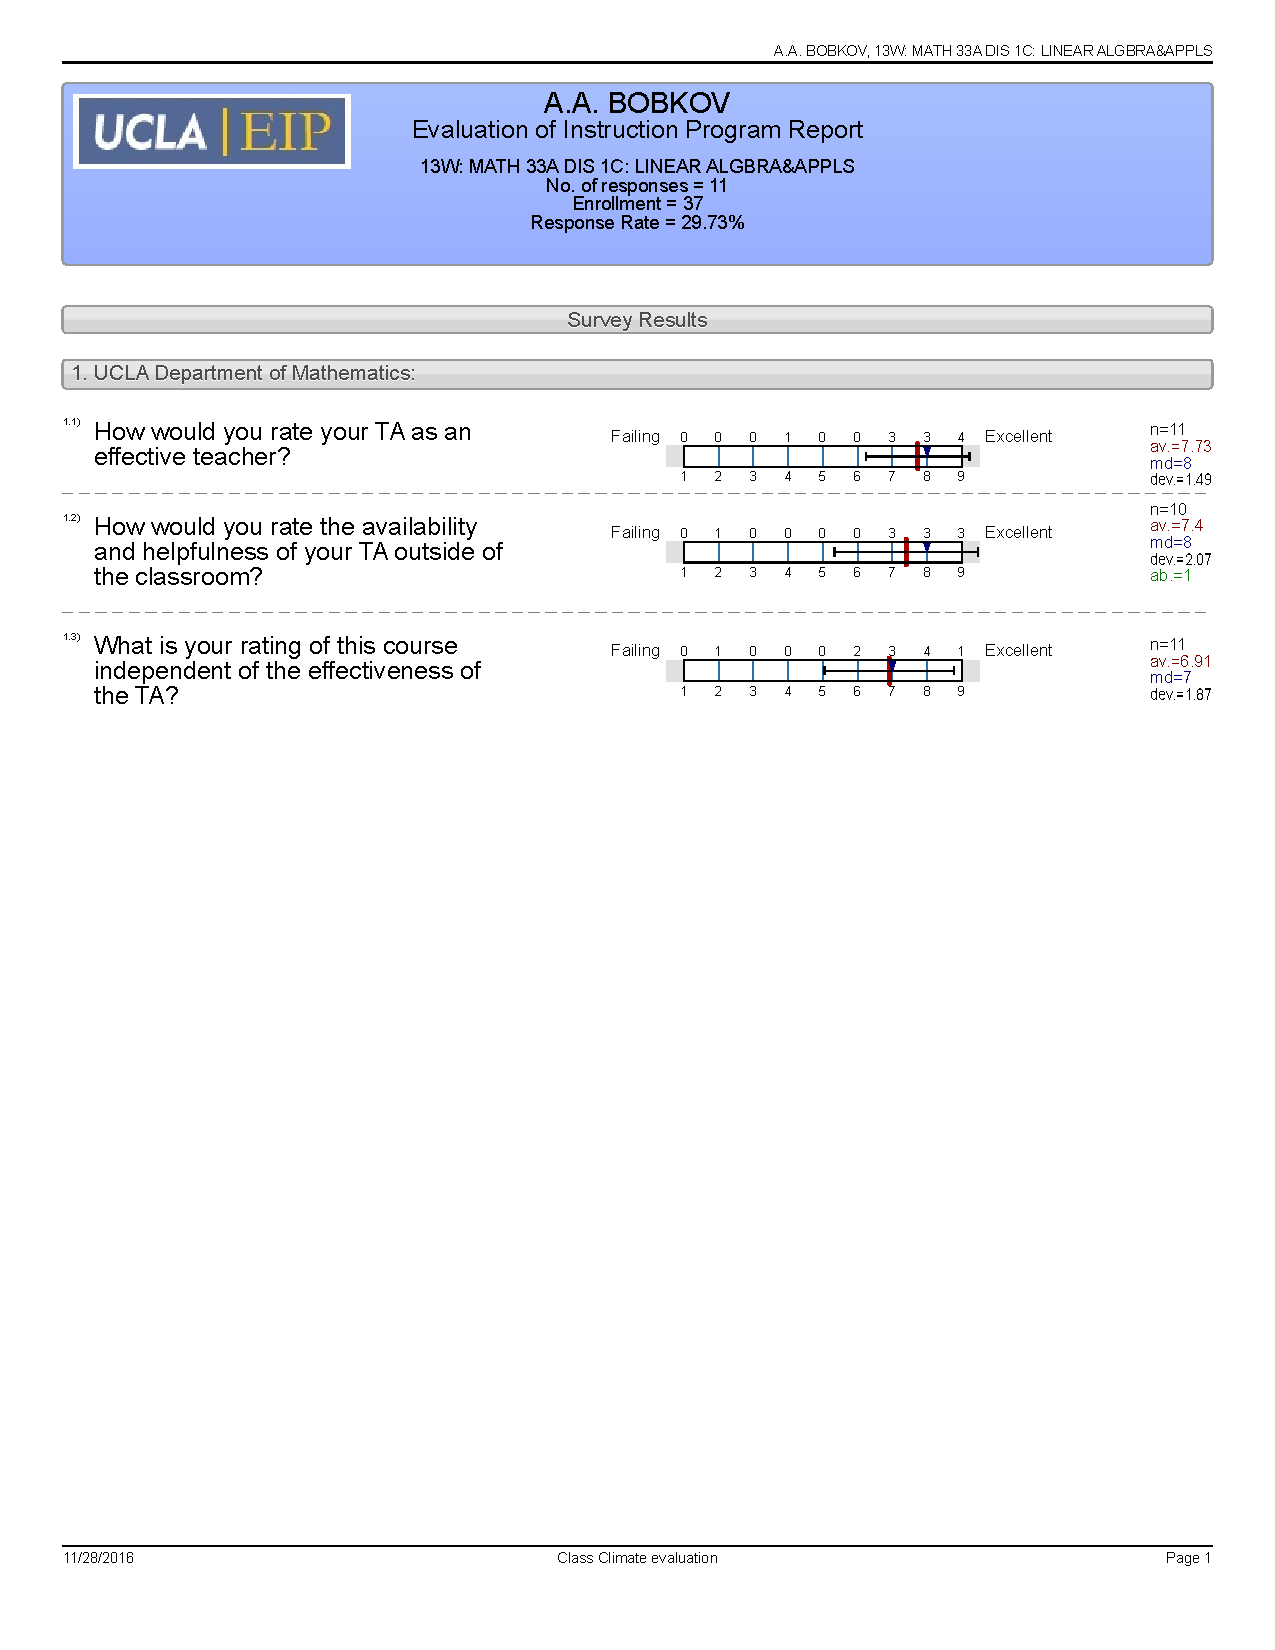
\includepdf[pages=-, offset=-80 0]{33a.pdf}
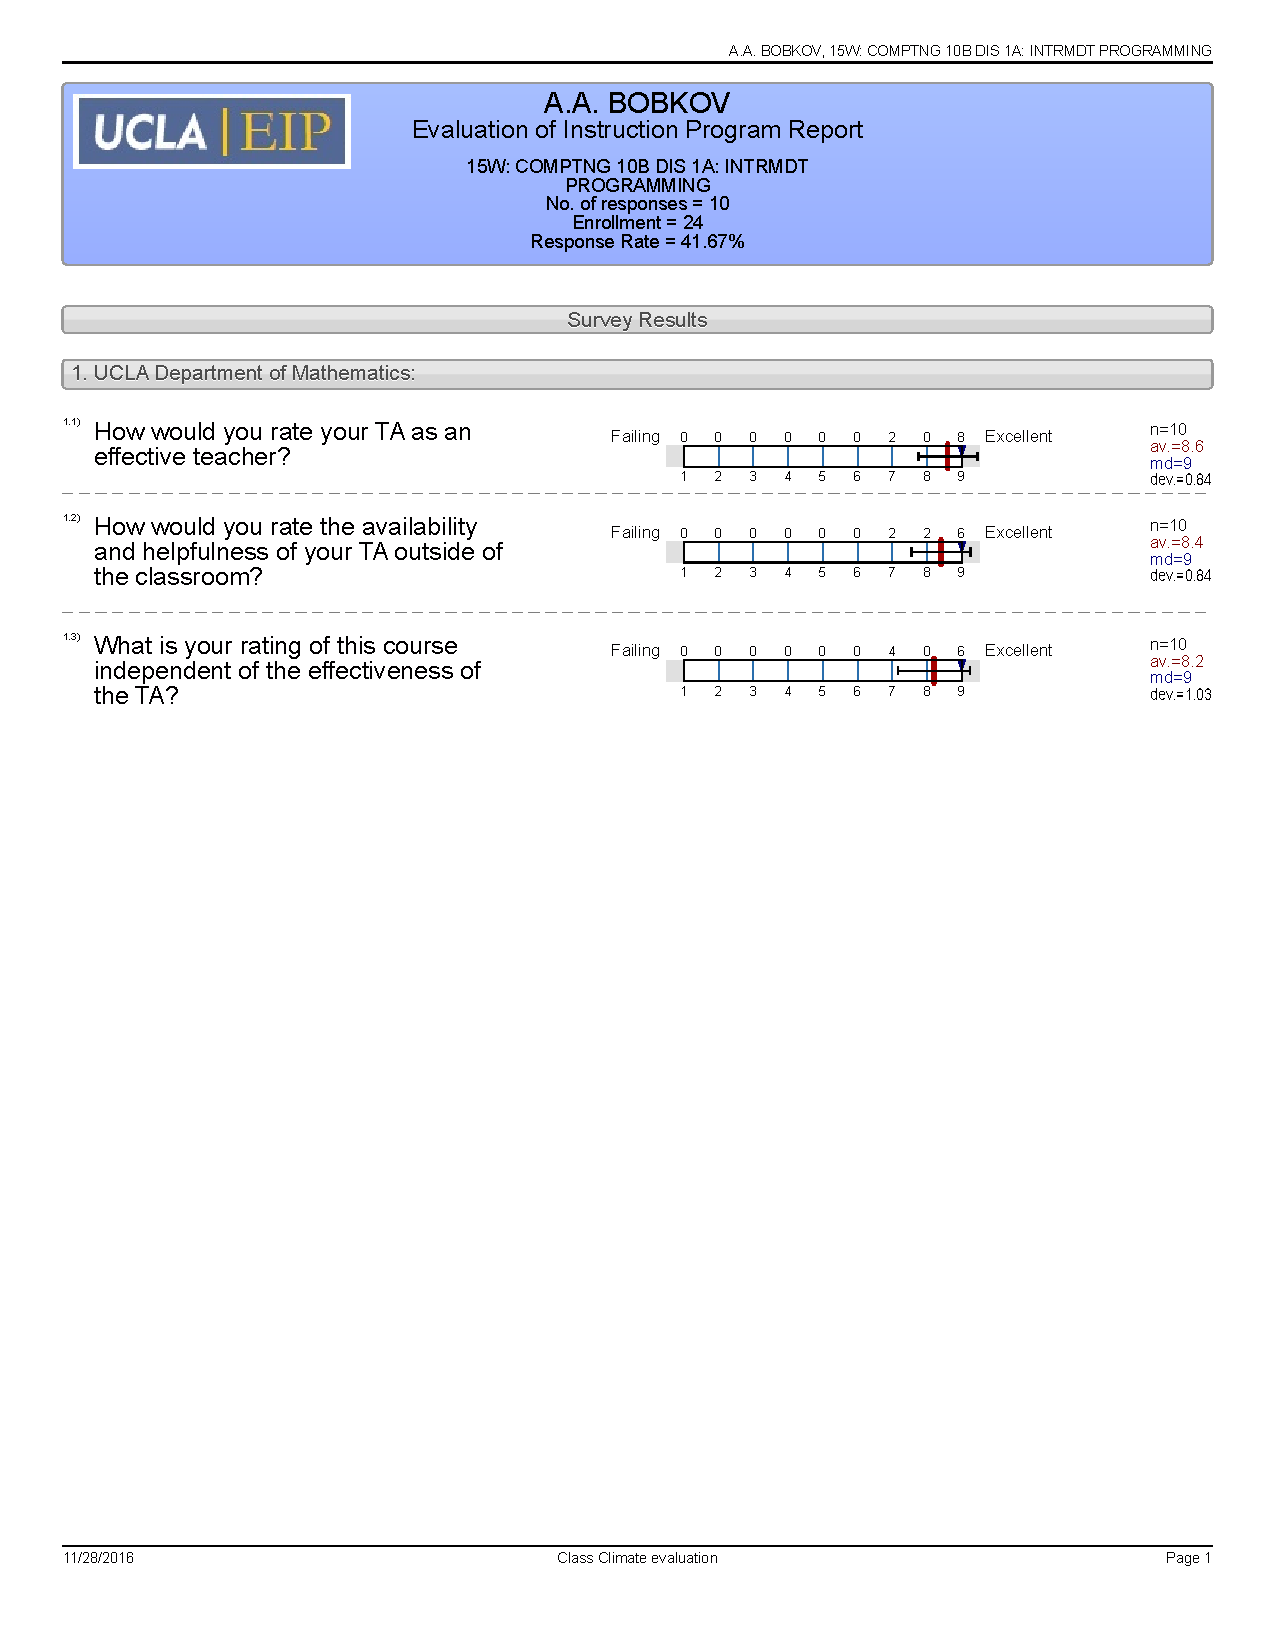
\includepdf[pages=-, offset=-80 0]{10b.pdf}
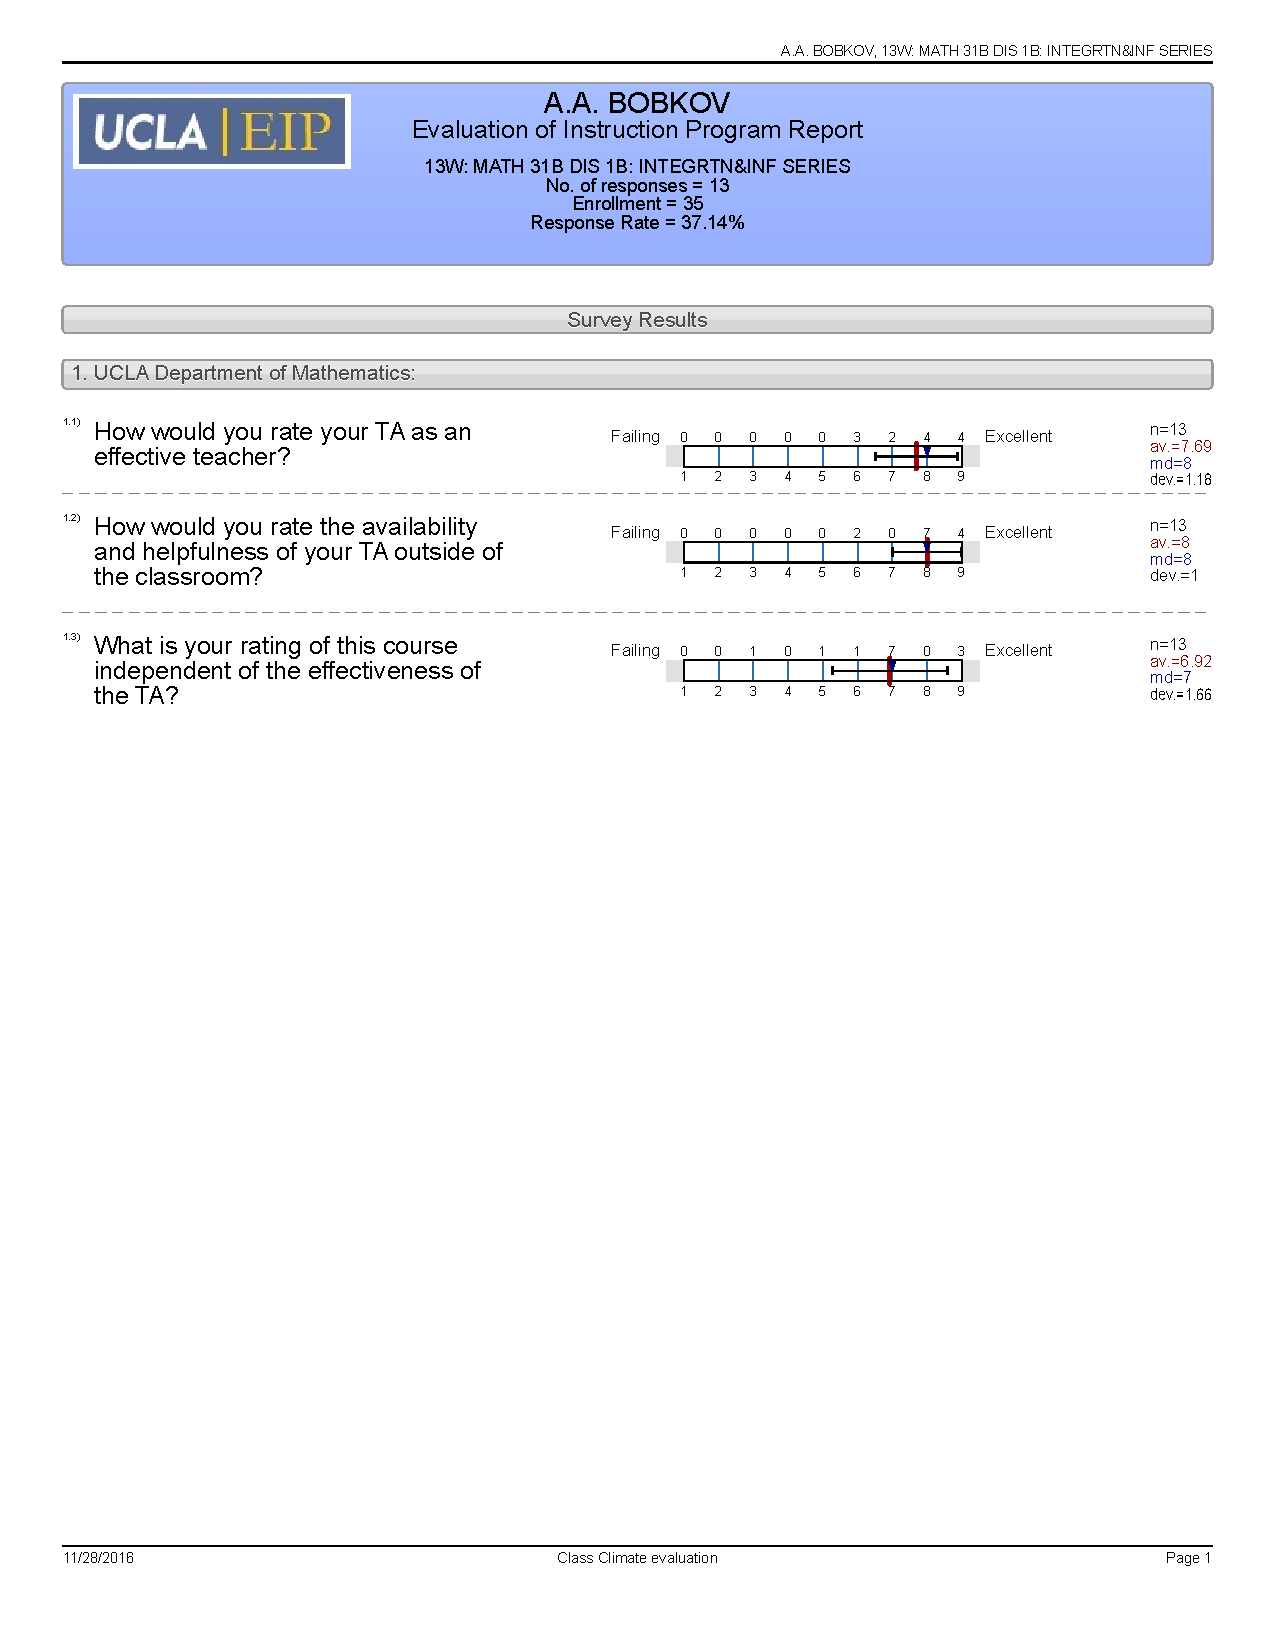
\includepdf[pages=-, offset=-80 0]{31b.pdf}
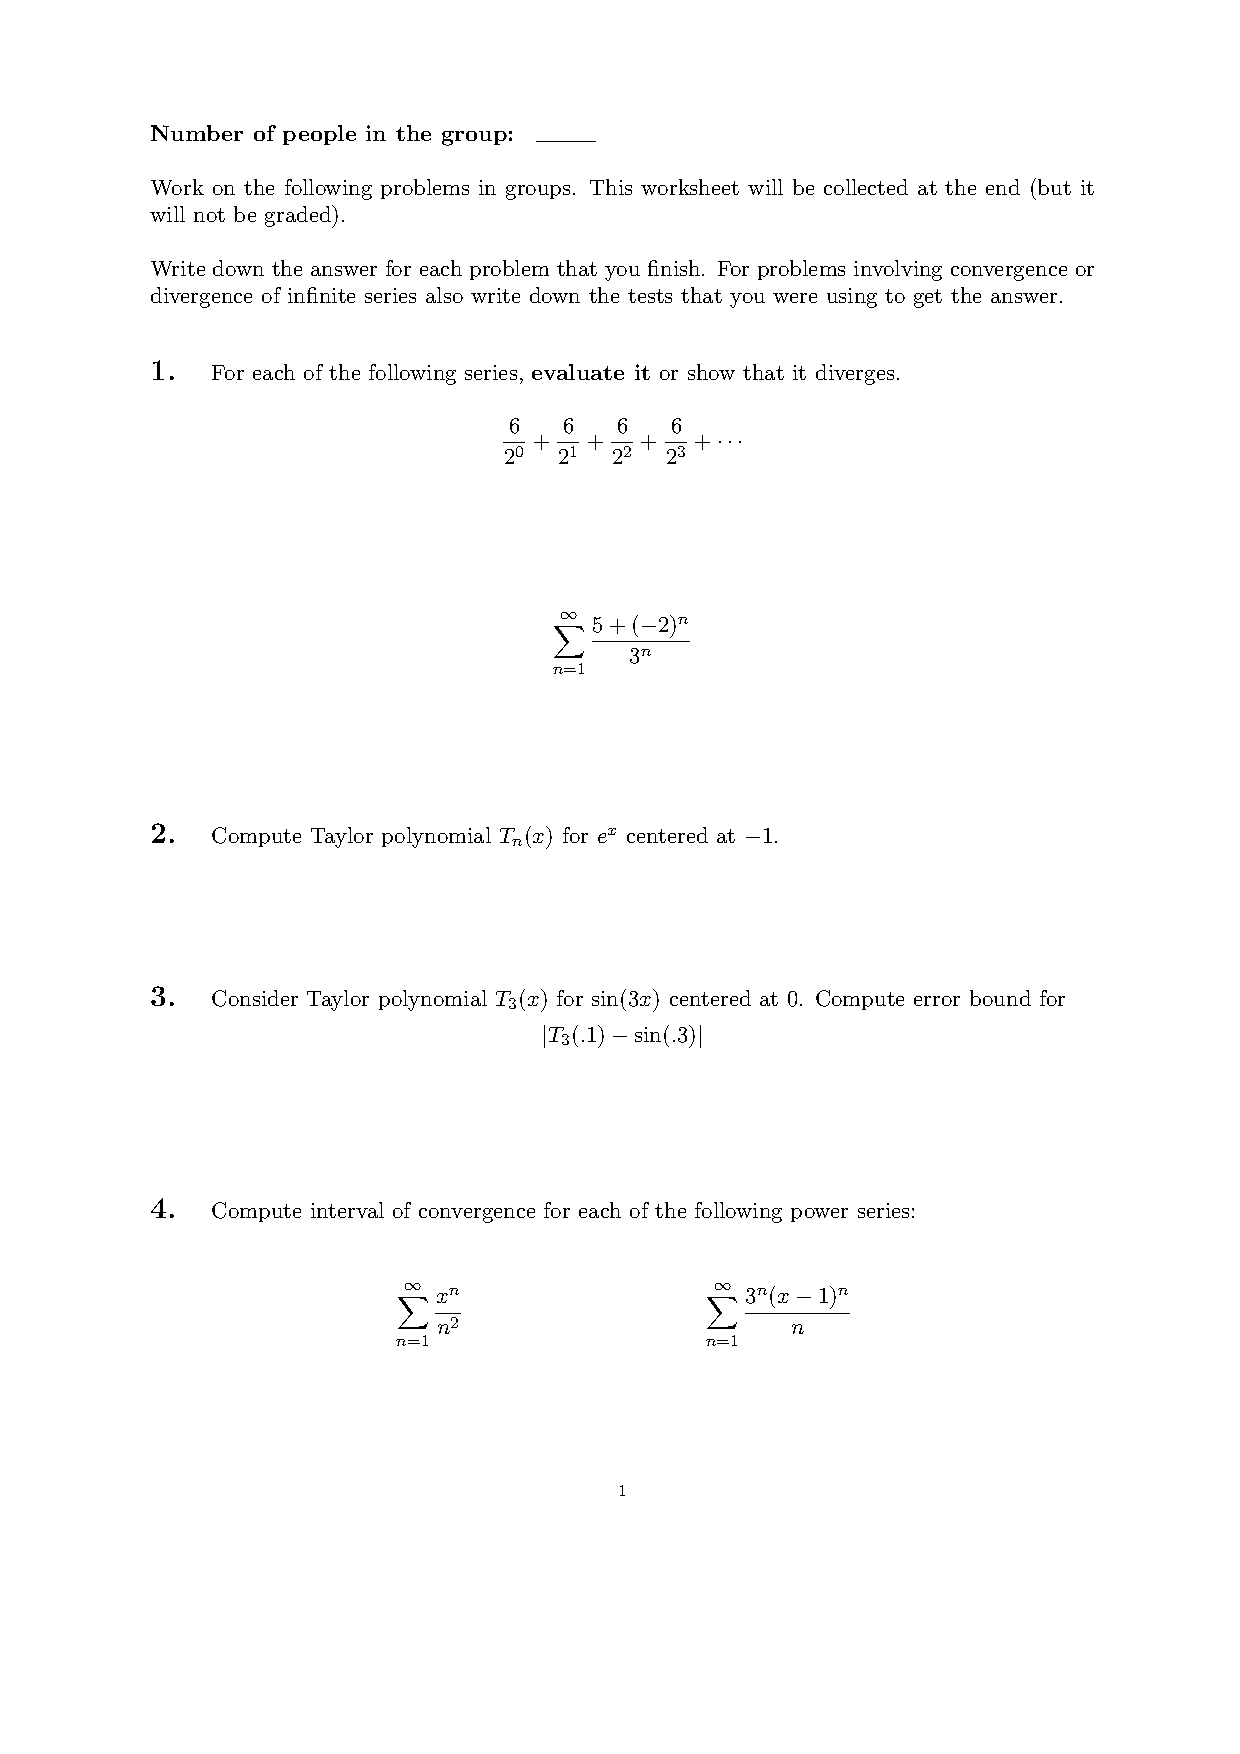
\includepdf[pages=-, offset=-80 0]{review.pdf}
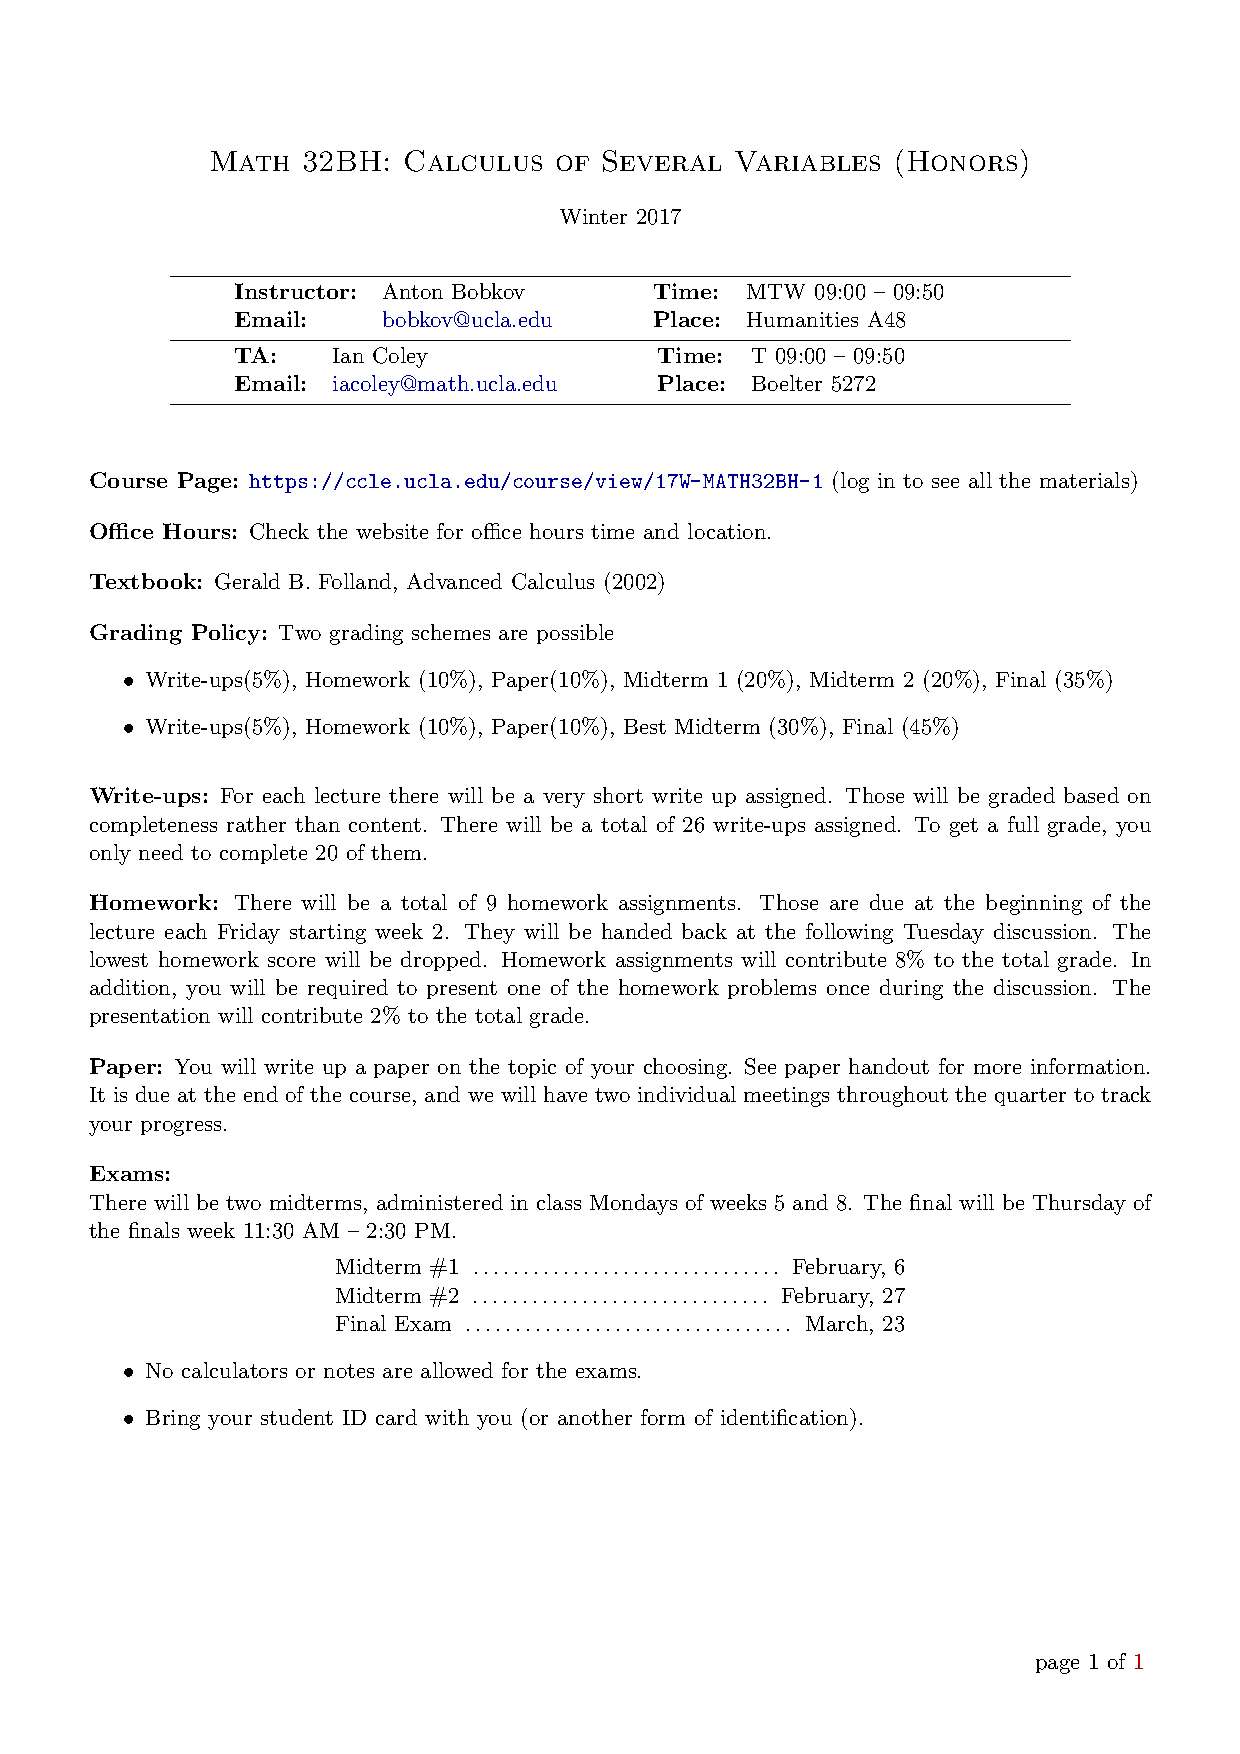
\includepdf[pages=-, offset=-80 0]{syllabus.pdf}
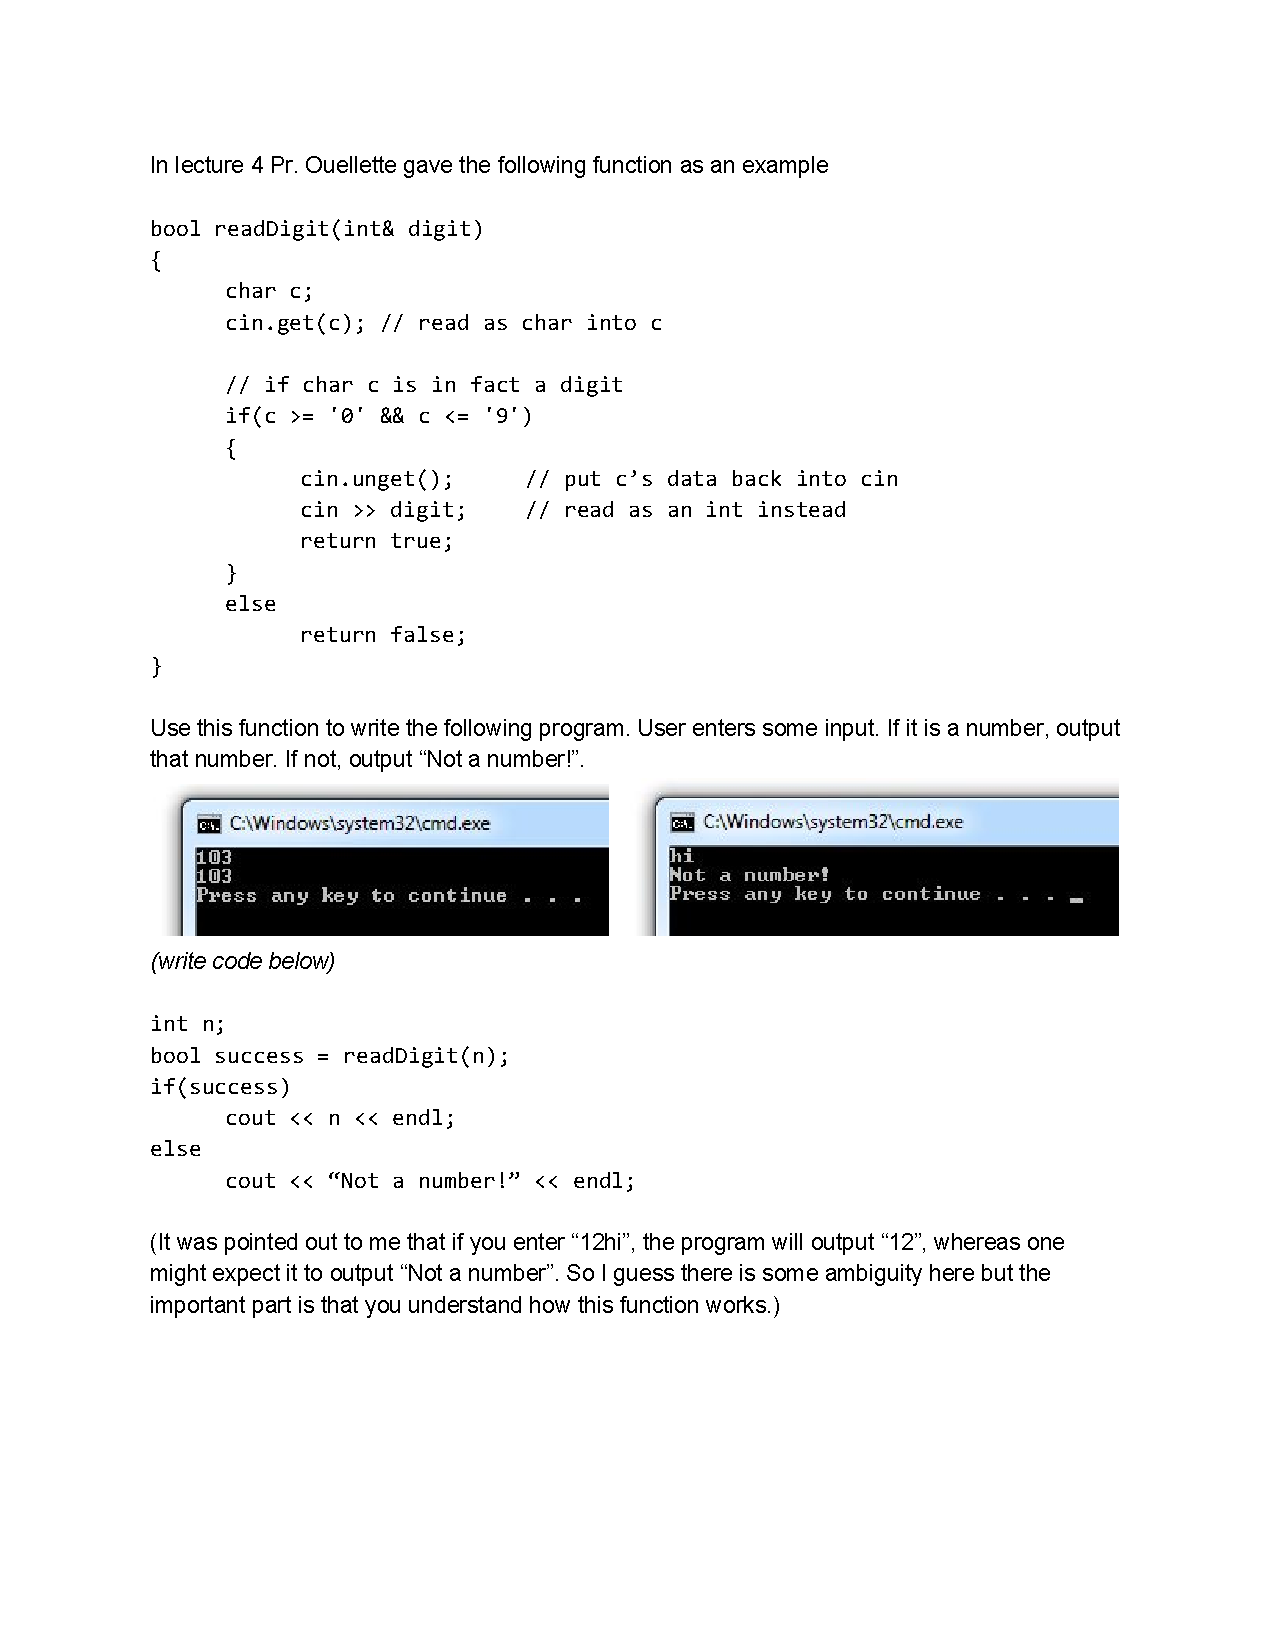
\includepdf[pages=-, offset=-80 0]{programming.pdf}
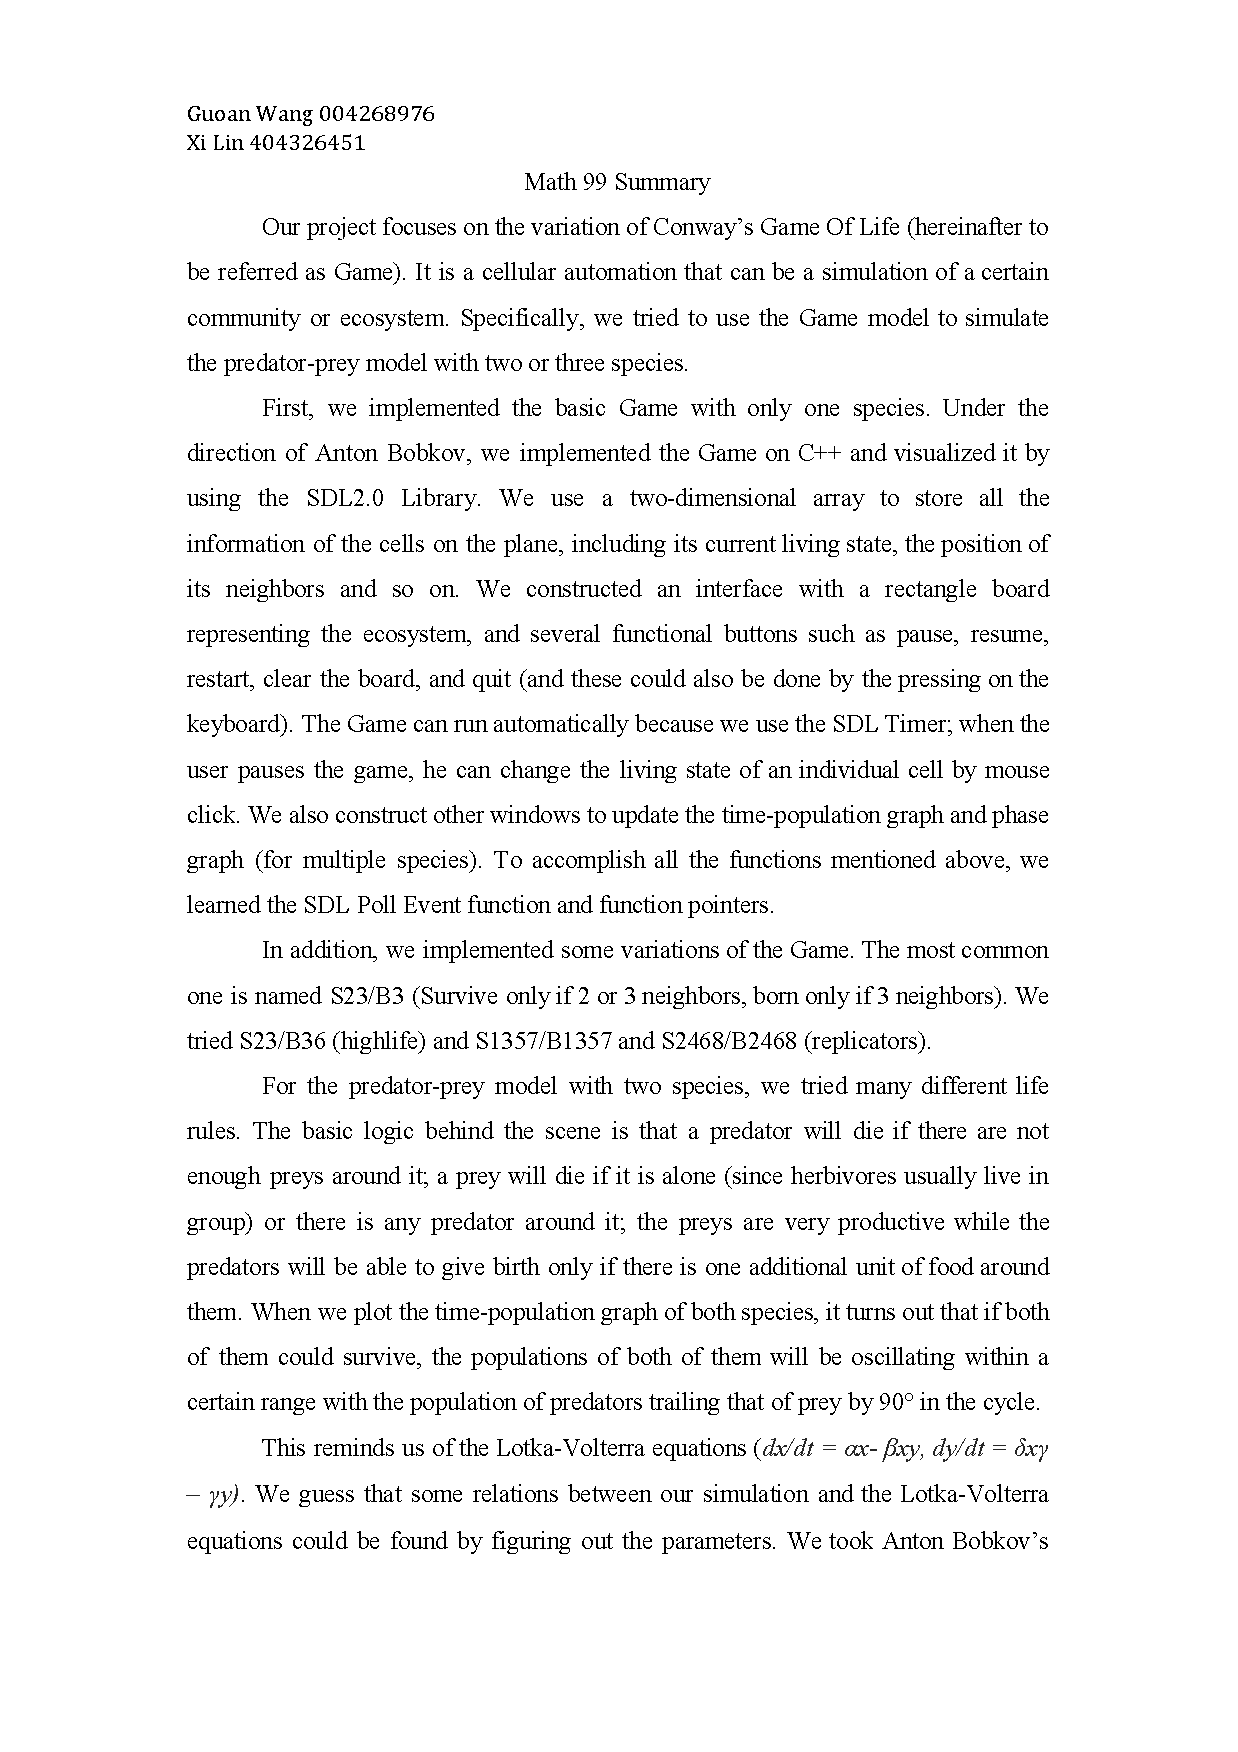
\includepdf[pages=-, offset=-80 0]{independent.pdf}
\end{document}
